		\section{Nombre: Bolas de nieve}\label{obs.bolasN}
	\subsection{Descripción}
	Conjunto de bolas de nieve, su característica es rígida. Posicionadas en un punto determinado, preferentemente alto. Este objeto cuenta con un área donde se detecta si ha pasado el jugador, de ser así las bolas de nieve caerán.
	\subsection{Esquema}
	Ver figura \ref{fig:bolasN}.
	\begin{figure}
		\centering
		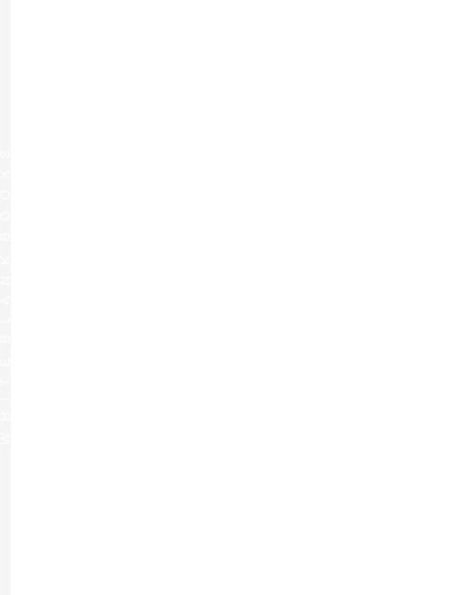
\includegraphics[height=0.2 \textheight]{Imagenes/bolasN}
		\caption{Sacos de cacao.}
		\label{fig:bolasN}
	\end{figure}